\subsection{3-2 GSCopy}

\subsubsection*{Shared Code}

\inputgroovy[label=GSCopy.groovy,firstline=5]{../ChapterExercises/src/c3/GSCopy.groovy}

\subsubsection{3-2-1 GSCopyA}

\subsubsection*{Code}

\inputgroovy[label=GSquaresA.groovy,firstline=6]{../ChapterExercises/src/c3/GSquaresA.groovy}
\inputgroovy[label=TestGSCopyA.groovy,firstline=6]{../ChapterExercises/src/c3/TestGSCopyA.groovy}

\subsubsection*{Results}

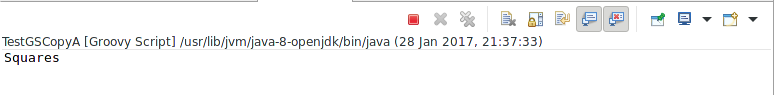
\includegraphics[width=\textwidth]{img/screenshots/3-2-1.png}

\paragraph{What happens?}

The application deadlocks and no data is printed.

\paragraph{Why does this happen?}

This happens because GSPairsA first writes to \mintinline{groovy}{outChannel0} which is read by GPlus.  After this GSPairsA writes to \mintinline{groovy}{outChannel1}, this value is read by GTail which discards the value.  GSPairsA then attempts to write to \mintinline{groovy}{outChannel0} however, because nothing has been written to GPlus's second input channel, the code locks at this write call.  To continue execution GSPairs must write to \mintinline{groovy}{outChanel1} however it is unable to do this as the two write calls are in series not parallel.


\subsubsection{3-2-2 GSCopyB}

\subsubsection*{Code}

\inputgroovy[label=GSquaresA.groovy,firstline=6]{../ChapterExercises/src/c3/GSquaresB.groovy}
\inputgroovy[label=TestGSCopyA.groovy,firstline=6]{../ChapterExercises/src/c3/TestGSCopyB.groovy}

\subsubsection*{Results}

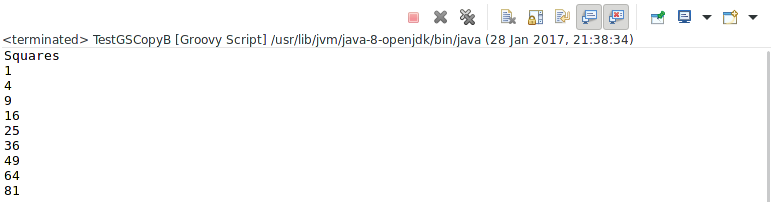
\includegraphics[width=\textwidth]{img/screenshots/3-2-2.png}
